\hypertarget{IndependenceTest_8c}{
\section{IndependenceTest.c File Reference}
\label{IndependenceTest_8c}\index{IndependenceTest.c@{IndependenceTest.c}}
}
{\tt \#include \char`\"{}party.h\char`\"{}}\par


Include dependency graph for IndependenceTest.c:\nopagebreak
\begin{figure}[H]
\begin{center}
\leavevmode
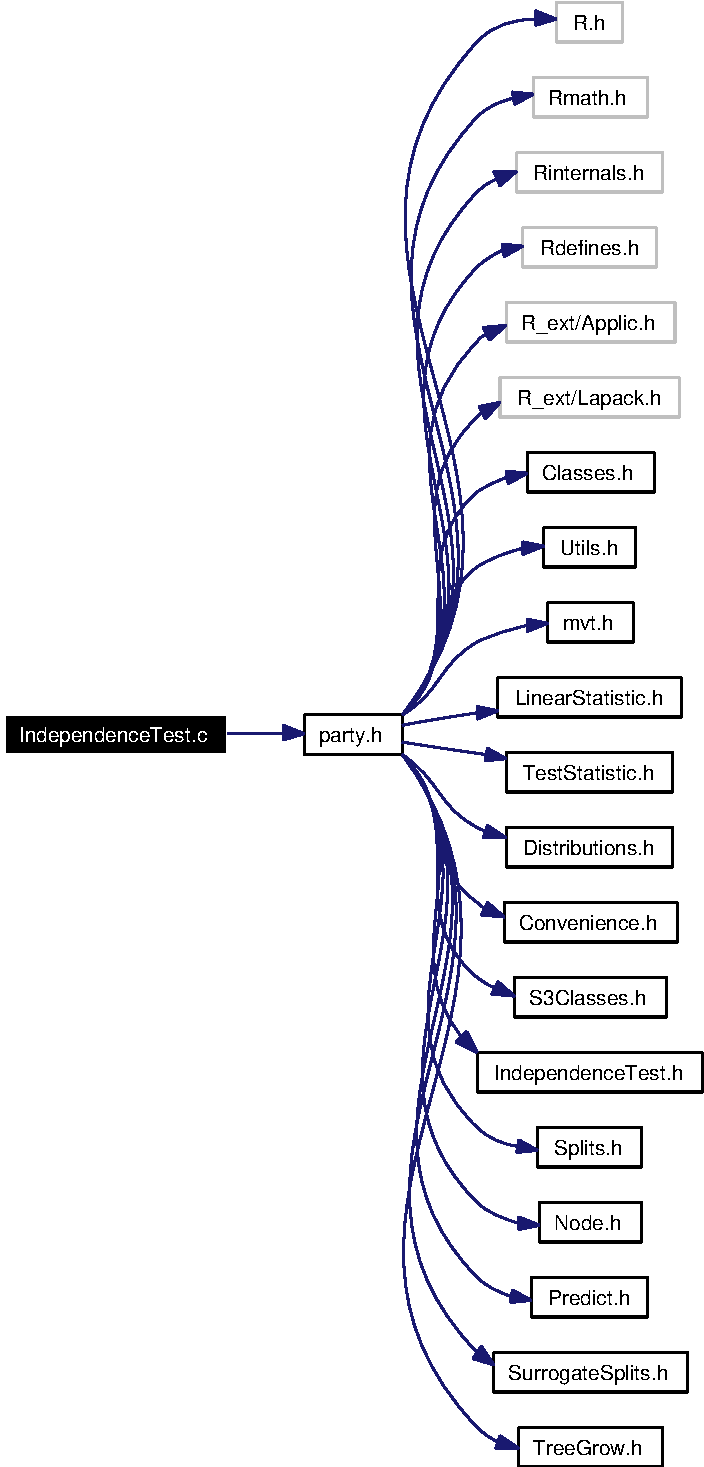
\includegraphics[width=420pt]{IndependenceTest_8c__incl}
\end{center}
\end{figure}
\subsection*{Functions}
\begin{CompactItemize}
\item 
void \hyperlink{IndependenceTest_8c_b02275a67ad210d96fed9864590ee3ef}{C\_\-TeststatPvalue} (const SEXP linexpcov, const SEXP varctrl, double $\ast$ans\_\-teststat, double $\ast$ans\_\-pvalue)
\item 
void \hyperlink{IndependenceTest_8c_d33688ffc38df769a95d6964e5bb193a}{C\_\-TeststatCriterion} (const SEXP linexpcov, const SEXP varctrl, double $\ast$ans\_\-teststat, double $\ast$ans\_\-criterion)
\item 
void \hyperlink{IndependenceTest_8c_e64c8d91a58113cee43788dc1663d645}{C\_\-IndependenceTest} (const SEXP x, const SEXP y, const SEXP weights, SEXP linexpcov, SEXP varctrl, SEXP ans)
\item 
SEXP \hyperlink{IndependenceTest_8c_aab8e2db15687b6b95f802dd1719ed54}{R\_\-IndependenceTest} (SEXP x, SEXP y, SEXP weights, SEXP linexpcov, SEXP varctrl)
\item 
void \hyperlink{IndependenceTest_8c_0de2357bd1d38058c0cfc68c3e743b34}{C\_\-GlobalTest} (const SEXP learnsample, const SEXP weights, SEXP fitmem, const SEXP varctrl, const SEXP gtctrl, const double minsplit, double $\ast$ans\_\-teststat, double $\ast$ans\_\-criterion)
\item 
SEXP \hyperlink{IndependenceTest_8c_f80dcff3dd9196b9f861fd83f4efa8ac}{R\_\-GlobalTest} (SEXP learnsample, SEXP weights, SEXP fitmem, SEXP varctrl, SEXP gtctrl)
\end{CompactItemize}


\subsection{Detailed Description}
Functions for variable selection in each node of a tree

\begin{Desc}
\item[Author:]\end{Desc}
\begin{Desc}
\item[Author]hothorn \end{Desc}
\begin{Desc}
\item[Date:]\end{Desc}
\begin{Desc}
\item[Date]2007-09-26 14:44:59 +0200 (Wed, 26 Sep 2007) \end{Desc}


Definition in file \hyperlink{IndependenceTest_8c-source}{IndependenceTest.c}.

\subsection{Function Documentation}
\hypertarget{IndependenceTest_8c_0de2357bd1d38058c0cfc68c3e743b34}{
\index{IndependenceTest.c@{IndependenceTest.c}!C\_\-GlobalTest@{C\_\-GlobalTest}}
\index{C\_\-GlobalTest@{C\_\-GlobalTest}!IndependenceTest.c@{IndependenceTest.c}}
\subsubsection{\setlength{\rightskip}{0pt plus 5cm}void C\_\-GlobalTest (const SEXP {\em learnsample}, \/  const SEXP {\em weights}, \/  SEXP {\em fitmem}, \/  const SEXP {\em varctrl}, \/  const SEXP {\em gtctrl}, \/  const double {\em minsplit}, \/  double $\ast$ {\em ans\_\-teststat}, \/  double $\ast$ {\em ans\_\-criterion})}}
\label{IndependenceTest_8c_0de2357bd1d38058c0cfc68c3e743b34}


Perform a global test on independence of a response and multiple inputs \par
 \begin{Desc}
\item[Parameters:]
\begin{description}
\item[{\em learnsample}]an object of class `LearningSample' \item[{\em weights}]case weights \item[{\em fitmem}]an object of class `TreeFitMemory' \item[{\em varctrl}]an object of class `VariableControl' \item[{\em gtctrl}]an object of class `GlobalTestControl' \item[{\em minsplit}]minimum sum of weights to proceed \item[{\em ans\_\-teststat}]return value; vector of test statistics \item[{\em ans\_\-criterion}]return value; vector of node criteria (adjusted) pvalues or raw test statistics \end{description}
\end{Desc}


Definition at line 129 of file IndependenceTest.c.

References AGGREGATED, BONFERRONI, C\_\-ExpectCovarInfluence(), C\_\-LinStatExpCov(), C\_\-LinStatExpCovMPinv(), C\_\-MonteCarlo(), C\_\-SampleNoReplace(), C\_\-tempweights(), C\_\-TeststatCriterion(), get\_\-dontuse(), get\_\-dontusetmp(), get\_\-mtry(), get\_\-ninputs(), get\_\-nobs(), get\_\-randomsplits(), get\_\-test\_\-trafo(), get\_\-teststat(), get\_\-testtype(), get\_\-tol(), get\_\-transformation(), get\_\-varmemory(), has\_\-missings(), MONTECARLO, ncol(), nrow(), PL2\_\-expcovinfSym, PL2\_\-inputsSym, PL2\_\-responsesSym, PL2\_\-sumweightsSym, TESTSTATISTIC, and UNIVARIATE.

Referenced by C\_\-Node(), and R\_\-GlobalTest().

Here is the call graph for this function:\nopagebreak
\begin{figure}[H]
\begin{center}
\leavevmode
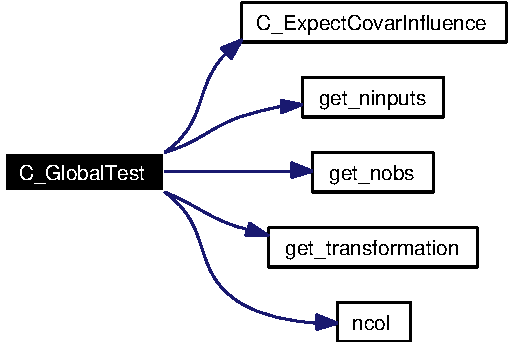
\includegraphics[width=420pt]{IndependenceTest_8c_0de2357bd1d38058c0cfc68c3e743b34_cgraph}
\end{center}
\end{figure}
\hypertarget{IndependenceTest_8c_e64c8d91a58113cee43788dc1663d645}{
\index{IndependenceTest.c@{IndependenceTest.c}!C\_\-IndependenceTest@{C\_\-IndependenceTest}}
\index{C\_\-IndependenceTest@{C\_\-IndependenceTest}!IndependenceTest.c@{IndependenceTest.c}}
\subsubsection{\setlength{\rightskip}{0pt plus 5cm}void C\_\-IndependenceTest (const SEXP {\em x}, \/  const SEXP {\em y}, \/  const SEXP {\em weights}, \/  SEXP {\em linexpcov}, \/  SEXP {\em varctrl}, \/  SEXP {\em ans})}}
\label{IndependenceTest_8c_e64c8d91a58113cee43788dc1663d645}


Test of independence between x and y \par
 \begin{Desc}
\item[Parameters:]
\begin{description}
\item[{\em x}]values of the transformation \item[{\em y}]values of the influence function \item[{\em weights}]case weights \item[{\em linexpcov}]an object of class `VariableControl' for T \item[{\em varctrl}]an object of class `VariableControl' \item[{\em ans;}]return value, a double vector (teststat, pvalue) \end{description}
\end{Desc}


Definition at line 78 of file IndependenceTest.c.

References C\_\-LinStatExpCov(), C\_\-LinStatExpCovMPinv(), C\_\-TeststatPvalue(), get\_\-teststat(), get\_\-tol(), ncol(), nrow(), and PL2\_\-expcovinfSym.

Referenced by R\_\-IndependenceTest().

Here is the call graph for this function:\nopagebreak
\begin{figure}[H]
\begin{center}
\leavevmode
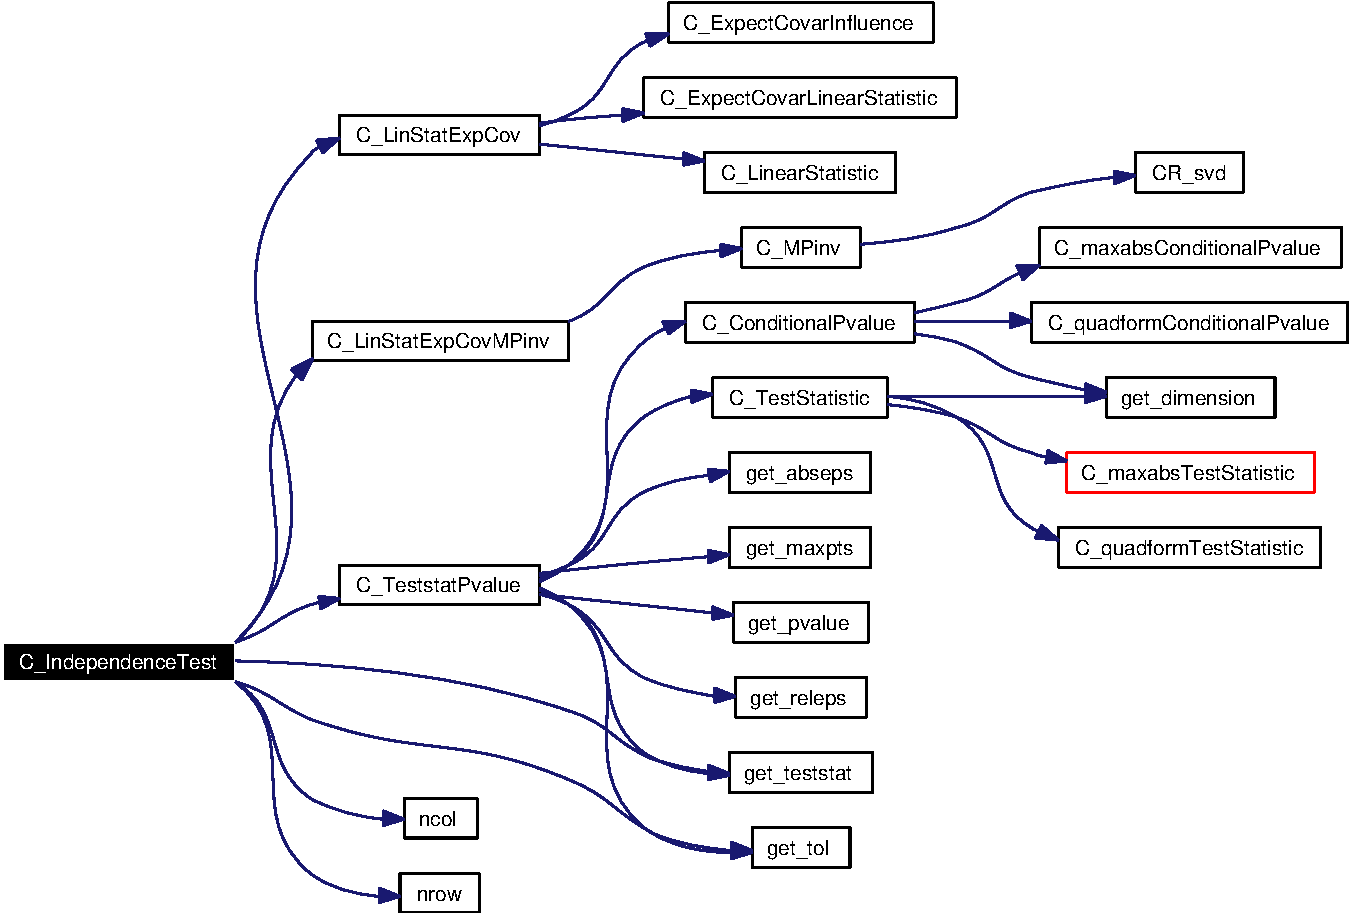
\includegraphics[width=420pt]{IndependenceTest_8c_e64c8d91a58113cee43788dc1663d645_cgraph}
\end{center}
\end{figure}
\hypertarget{IndependenceTest_8c_d33688ffc38df769a95d6964e5bb193a}{
\index{IndependenceTest.c@{IndependenceTest.c}!C\_\-TeststatCriterion@{C\_\-TeststatCriterion}}
\index{C\_\-TeststatCriterion@{C\_\-TeststatCriterion}!IndependenceTest.c@{IndependenceTest.c}}
\subsubsection{\setlength{\rightskip}{0pt plus 5cm}void C\_\-TeststatCriterion (const SEXP {\em linexpcov}, \/  const SEXP {\em varctrl}, \/  double $\ast$ {\em ans\_\-teststat}, \/  double $\ast$ {\em ans\_\-criterion})}}
\label{IndependenceTest_8c_d33688ffc38df769a95d6964e5bb193a}


Computes the test statistic and the node criterion \par
 \begin{Desc}
\item[Parameters:]
\begin{description}
\item[{\em linexpcov}]an object of class `LinStatExpectCovar' \item[{\em varctrl}]an object of class `VariableControl' \item[{\em ans\_\-teststat;}]return value, the test statistic \item[{\em ans\_\-criterion;}]return value, thep-value \end{description}
\end{Desc}


Definition at line 53 of file IndependenceTest.c.

References C\_\-TeststatPvalue(), and get\_\-pvalue().

Referenced by C\_\-GlobalTest(), and C\_\-MonteCarlo().

Here is the call graph for this function:\nopagebreak
\begin{figure}[H]
\begin{center}
\leavevmode
\includegraphics[width=420pt]{IndependenceTest_8c_d33688ffc38df769a95d6964e5bb193a_cgraph}
\end{center}
\end{figure}
\hypertarget{IndependenceTest_8c_b02275a67ad210d96fed9864590ee3ef}{
\index{IndependenceTest.c@{IndependenceTest.c}!C\_\-TeststatPvalue@{C\_\-TeststatPvalue}}
\index{C\_\-TeststatPvalue@{C\_\-TeststatPvalue}!IndependenceTest.c@{IndependenceTest.c}}
\subsubsection{\setlength{\rightskip}{0pt plus 5cm}void C\_\-TeststatPvalue (const SEXP {\em linexpcov}, \/  const SEXP {\em varctrl}, \/  double $\ast$ {\em ans\_\-teststat}, \/  double $\ast$ {\em ans\_\-pvalue})}}
\label{IndependenceTest_8c_b02275a67ad210d96fed9864590ee3ef}


Computes the test statistic and, if requested, the corresponding P-value for a linear statistic \par
 \begin{Desc}
\item[Parameters:]
\begin{description}
\item[{\em linexpcov}]an object of class `LinStatExpectCovar' \item[{\em varctrl}]an object of class `VariableControl' \item[{\em ans\_\-teststat;}]return value, the test statistic \item[{\em ans\_\-pvalue;}]return value, the p-value \end{description}
\end{Desc}


Definition at line 21 of file IndependenceTest.c.

References C\_\-ConditionalPvalue(), C\_\-TestStatistic(), get\_\-abseps(), get\_\-maxpts(), get\_\-pvalue(), get\_\-releps(), get\_\-teststat(), and get\_\-tol().

Referenced by C\_\-IndependenceTest(), and C\_\-TeststatCriterion().

Here is the call graph for this function:\nopagebreak
\begin{figure}[H]
\begin{center}
\leavevmode
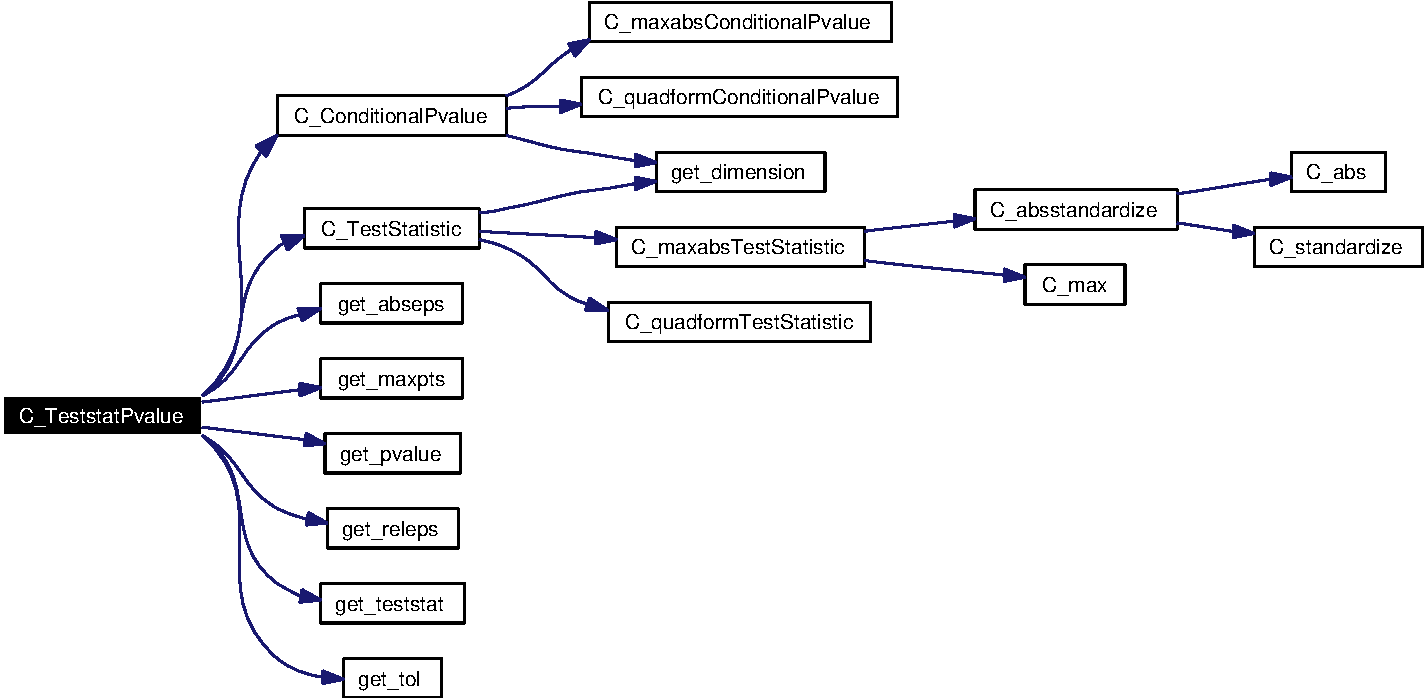
\includegraphics[width=354pt]{IndependenceTest_8c_b02275a67ad210d96fed9864590ee3ef_cgraph}
\end{center}
\end{figure}
\hypertarget{IndependenceTest_8c_f80dcff3dd9196b9f861fd83f4efa8ac}{
\index{IndependenceTest.c@{IndependenceTest.c}!R\_\-GlobalTest@{R\_\-GlobalTest}}
\index{R\_\-GlobalTest@{R\_\-GlobalTest}!IndependenceTest.c@{IndependenceTest.c}}
\subsubsection{\setlength{\rightskip}{0pt plus 5cm}SEXP R\_\-GlobalTest (SEXP {\em learnsample}, \/  SEXP {\em weights}, \/  SEXP {\em fitmem}, \/  SEXP {\em varctrl}, \/  SEXP {\em gtctrl})}}
\label{IndependenceTest_8c_f80dcff3dd9196b9f861fd83f4efa8ac}


R-interface to C\_\-GlobalTest \par
 \begin{Desc}
\item[Parameters:]
\begin{description}
\item[{\em learnsample}]an object of class `LearningSample' \item[{\em weights}]case weights \item[{\em fitmem}]an object of class `TreeFitMemory' \item[{\em varctrl}]an object of class `VariableControl' \item[{\em gtctrl}]an object of class `GlobalTestControl' \end{description}
\end{Desc}


Definition at line 272 of file IndependenceTest.c.

References C\_\-GlobalTest(), and get\_\-ninputs().

Here is the call graph for this function:\nopagebreak
\begin{figure}[H]
\begin{center}
\leavevmode
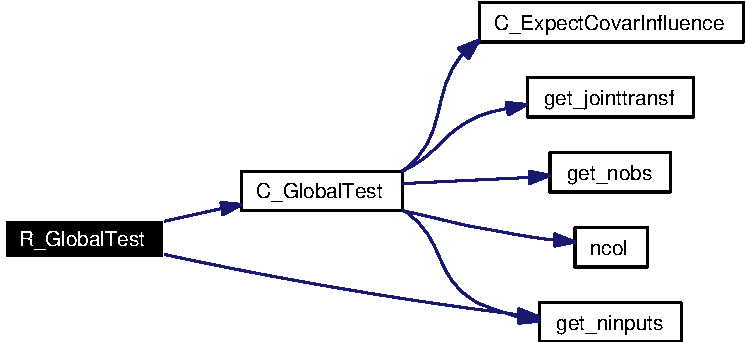
\includegraphics[width=420pt]{IndependenceTest_8c_f80dcff3dd9196b9f861fd83f4efa8ac_cgraph}
\end{center}
\end{figure}
\hypertarget{IndependenceTest_8c_aab8e2db15687b6b95f802dd1719ed54}{
\index{IndependenceTest.c@{IndependenceTest.c}!R\_\-IndependenceTest@{R\_\-IndependenceTest}}
\index{R\_\-IndependenceTest@{R\_\-IndependenceTest}!IndependenceTest.c@{IndependenceTest.c}}
\subsubsection{\setlength{\rightskip}{0pt plus 5cm}SEXP R\_\-IndependenceTest (SEXP {\em x}, \/  SEXP {\em y}, \/  SEXP {\em weights}, \/  SEXP {\em linexpcov}, \/  SEXP {\em varctrl})}}
\label{IndependenceTest_8c_aab8e2db15687b6b95f802dd1719ed54}


R-interface to C\_\-IndependenceTest \par
 \begin{Desc}
\item[Parameters:]
\begin{description}
\item[{\em x}]values of the transformation \item[{\em y}]values of the influence function \item[{\em weights}]case weights \item[{\em linexpcov}]an object of class `VariableControl' for T \item[{\em varctrl}]an object of class `VariableControl' \end{description}
\end{Desc}


Definition at line 105 of file IndependenceTest.c.

References C\_\-IndependenceTest().

Here is the call graph for this function:\nopagebreak
\begin{figure}[H]
\begin{center}
\leavevmode
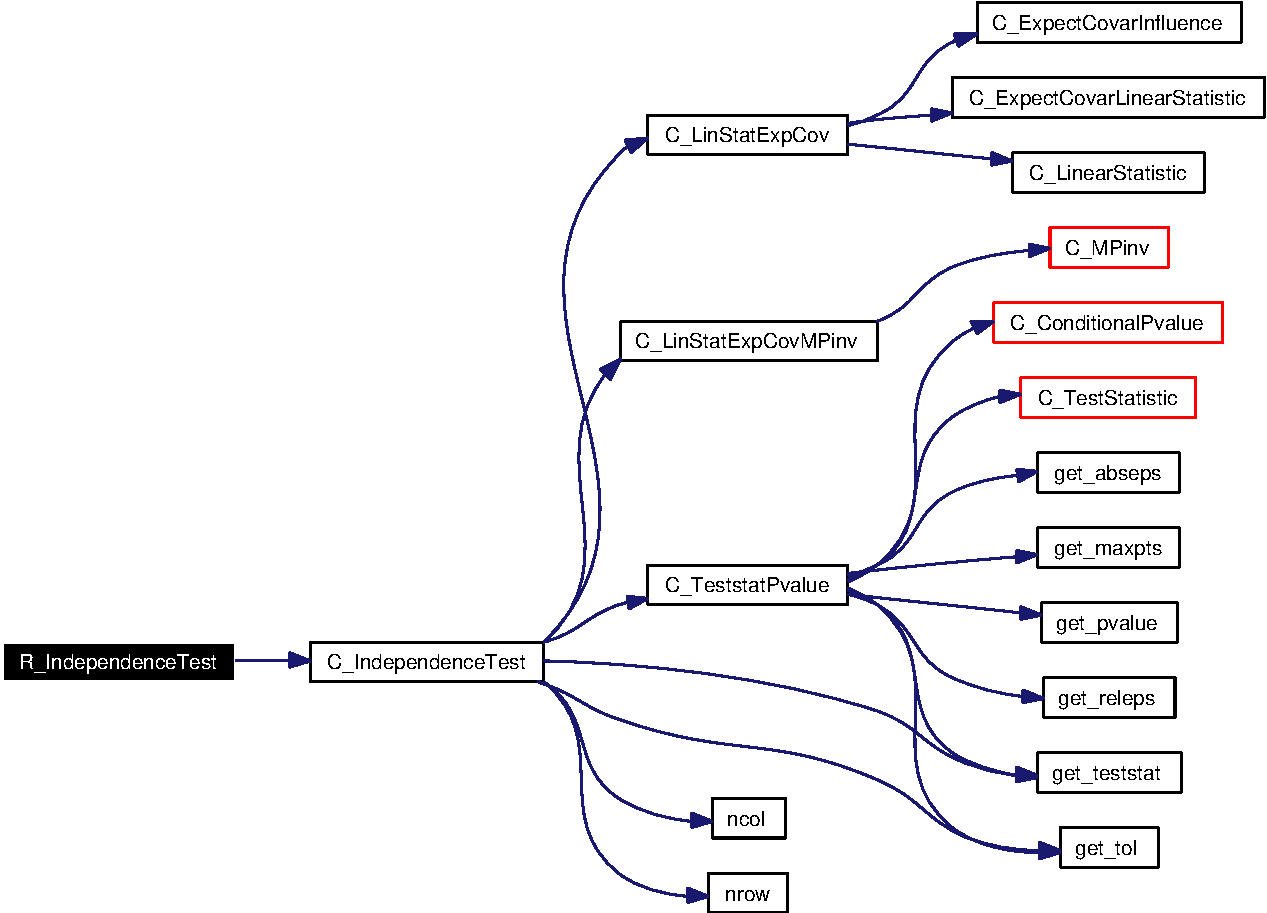
\includegraphics[width=420pt]{IndependenceTest_8c_aab8e2db15687b6b95f802dd1719ed54_cgraph}
\end{center}
\end{figure}
